\chapter{Metodologia} % (fold)
\label{cha:metodologia}

Será apresentado a seguir um descritivo das etapas que serão necessárias para guiar e, por consequência, validar o presente trabalho.
Podemos resumir os estágios em: (i) modelagem dos problemas propostos, (ii) estudo das soluções existentes para tais problema, (iii) experimentação de novas abordagens considerando ambientes reais e simulados, e (iv) expor as características que fazem desta nova solução relevante, melhor ou não em relação às demais.

A revisão bibliográfica foi focada em pesquisas que envolvam o controle e coordenação de robôs heterogêneos em tarefas que necessitem de um ou mais agentes para sua realização, como a de exploração, busca e resgate e principalmente no transporte cooperativo, que é foco deste trabalho.

% Imagem
A Figura~\ref{fig:geral_diagram} apresenta uma visão geral das etapas deste processo. Baseado em um mapa pré-estabelecido e um conjunto de objetos a serem transportados (descritos por suas características, como dimensões e peso), o sistema proposto deve produzir um trajeto que levará os alvos para seus determinados destinos. Seguindo o fluxo, vemos que este planejamento é a entrada para o sistema de coordenação que, juntamente com os recursos robóticos disponíveis, deve gerenciar a equipe de modo a cumprir a tarefa demandada.

\img{001-DiagramaGeral.png}{0.55\textwidth}{Esquema representante da organização do sistema proposto, dividido nos passos de planejamento de caminho baseado nos objetos, seguido pela coordenação da equipe de robôs para executar a tarefa de transporte.}{geral_diagram}

\section{Planejamento de Caminho do Objeto} % (fold)
\label{sub:planejamento_de_caminho_do_objeto}

Para o Problema 1 (Planejamento de Caminho do Objeto) pretende-se estudar como a movimentação do objeto pelo ambiente é influenciada pelas suas dimensões e peso. Inicialmente, será considerado que o objeto possui liberdade suficiente para se mover sozinho pelo ambiente, deste modo, será criado um caminho plausível para seu deslocamento. Após esta etapa, agora considerando não somente as dimensões do objetos, mas também dos robôs que poderiam executar a tarefa, a trajetória criada será modificada e aprimorada se necessário para conter estas novas restrições.

A criação do caminho a ser percorrido pelo objeto será realizada através da combinação entre técnicas de discretização do ambiente e as poses válidas considerando os obstáculos nele presente.
Para tanto, uma mapa será dividido em células seguindo o método de Mapa Discreto, segregando células ocupadas das livres.
Considerando uma função de distância entre a pose inicial e final, como a distância Euclidiana ou de Manhattan, podemos executar algoritmos como o $A^{*}$ para determinar o menor caminho entre as mesmas.
Partiremos das poses inicial e final, procurando por um ponto de encontro, assim esperamos diminuir o tempo necessário para gerar este trajeto.

Considerando os diversos ambientes em que este sistema pode ser aplicado, há o caso no qual o objeto não pode ser deslocado somente por via terrestre, condição na qual a pose final está cercada por obstáculos. Neste caso, os trajetos intermediários (partindo da pose inicial e final) serão interligados como uma linha reta, pois é o menor caminho possível.

Após a concepção do caminho a ser realizado, o mesmo será segmentado baseando-se principalmente na descontinuidade do trajeto principal, por exemplo, no caso do caminho passar por um obstáculo. Estas marcações servirão para alocação de tarefas dentro da equipe de agentes. A Figura~\ref{fig:planejamento_objeto} exemplifica esta estratégia quando em (a) temos um mapa sem obstáculos entre as poses, deste modo temos um trajeto contínuo que possivelmente será realizado por somente um tipo de agente, já em (b) o caminho planejado é segmentado mediante a presença de obstáculos, este trajeto será realizado por agentes que possam sobrepujar estas restrições.

\begin{figure}[!h]
  \centering

  \subfloat[]{
    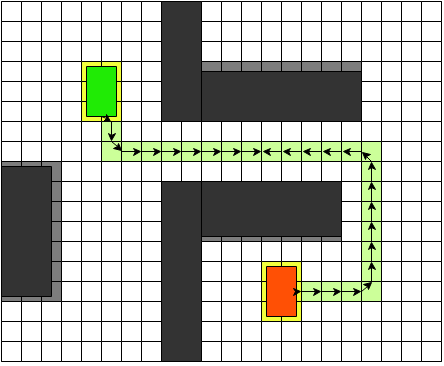
\includegraphics[width=0.48\textwidth]{img/005-DiagramaProblema1-Explain_1.png}
  }
  \subfloat[] {
    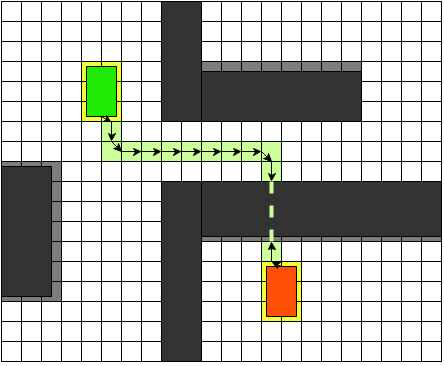
\includegraphics[width=0.48\textwidth]{img/005-DiagramaProblema1-Explain_2.png}
  }

  \caption{Planejamento de Caminhos para o Objeto: (a) mapa sem obstáculos entre a pose inicial e final e (b) mapa com obstáculos entre estas poses.}
  \label{fig:planejamento_objeto}

\end{figure}

% subsection planejamento_de_caminho_do_objeto (end)

\section{Coordenação dos Robôs} % (fold)
\label{sub:coordena_o_dos_rob_s}

O Problema 2 (Coordenação dos Robôs) levará em consideração a rota gerada, e terá como principal foco estudar como esta influencia na alocação de tarefa entre as equipes de robôs (aéreos e terrestres), pois em certo momento a trajetória pode necessitar de recursos que somente um tipo de agente é capaz de proporcionar, ou mesmo somente uma subequipe esta apta.

A alocação de tarefas dentro da equipe seguirá principalmente o caráter de recursos necessários para cada trecho. Uma função de custo associado ao trecho servirá de base para esta distribuição. A Equação~\ref{funcao_custo} apresenta uma formulação para esta função de custo,

\begin{equation}
  \mbox{custo}(t, r) = \mbox{tempo}(t) + \mbox{distância}(t) + \mbox{energia}(t, r).
  \label{funcao_custo}
\end{equation}

A função descrita pela Equação~\ref{funcao_custo} associa a estimativa de tempo necessário para movimentação no sub-trajeto $t$, a distância baseada no mapa discreto bem como a estimativa de gasto energético de um determinado agente $r$ ou uma subequipe de agentes. Mediante esta função, podemos destacar do quadro de robôs, aquela formação que tem menor custo associado. Se mais de um arranjo for capaz de realizar a tarefa com o menor custo, aquela que estiver mais próximo ao ponto de execução. Uma ilustração da alocação baseada nesta função é demonstrada na Figura~\ref{fig:cost_function}:

\img{cost_function.png}{\textwidth}{Gráfico de exemplo da Função de Custo para três agentes dado um trajeto subdividido em 4 etapas.}{cost_function}

A Figura~\ref{fig:cost_function} demonstra uma saída da Equação de Custo (\ref{funcao_custo}) para três agentes com capacidades diferentes baseado em um trajeto subdividido em quatro etapas. Podemos perceber que para as etapas 2 e 3, alocaríamos o Agente 2, pois possui o menor custo associado, os demais sub-trajetos 1 e 4 são dados ao Agentes 1 e 3 respectivamente.

Após a alocação de tarefas dentre os agentes, podemos realizar a coordenação dos mesmos seguindo técnicas mais simplistas, como o controle Centralizado, que garante uma visão geral do sistema a partir de um só ponto, porém, é intensão deste trabalho promover um meio totalmente Descentralizado para tal coordenação, principalmente por promover escalabilidade ao sistema, ao contrário do outro método citado.

% Após a alocação de tarefas, podemos realizar a coordenação dos agentes seguindo algumas técnicas, como o controle Centralizado primeiramente,
% por se tratar de uma estratégia que garante um melhor controle dos agentes, mas com a intenção de um controle totalmente Descentralizado, por promover escalabilidade ao sistema.

\section{Localização} % (fold)
\label{sec:localiza_o}

Para a localização tanto dos objetos quanto dos agentes no cenário, serão utilizados métodos que utilizam marcadores visuais para situar estes elementos, para tanto os principais sensores utilizados neste trabalho serão câmeras RGB. Segue a descrição da técnica empregada:

\begin{itemize}
  \item \textbf{Localização dos Agentes:} A localização dos robôs será baseada no uso de pontos de referência no formato de marcadores pelo cenário. Tanto os agentes terrestres quanto os aéreos usarão este tipo de localização. Marcadores utilizados serão no formato de \emph{QR Codes} ou \emph{Fiduciais}.

  \item \textbf{Localização dos Objetos:} De maneira similar, cada objeto no cenário possuirá marcadores em suas faces, para sua detecção e localização. Além desta marcação, agentes terrestres podem utilizar sensores \emph{laser} para detectar a presença de obstáculos durante sua movimentação.

\end{itemize}

% chapter metodologia (end)
